\section{System architecture}
The Energy Lens application aims to approximate the vision described in section~\ref{sec:vision}.  For our initial
attempt, we tagged items in a building with QR codes and allowed users to 1) register new items and tag
them with QR codes they can print from the Energy Lens site, 2) tell us which meters are attached to which items,
3) scan individual item to view their load curve over a 24-hour period.

The architecture consists of three layers: the sensing and tag layer, the data management and processing layer, and the application
layer.  In this section we discuss each layer and their most important components.  Each layer in the architecture
is carefully design to work on a real deployment with live users.  In deploying the application in a real building, we ran
into various issues that informed our design.  For example, \emph{QR code reading times vary substantially across phones
and lighting conditions}.  You must design for the least-common demoninator in terms of camera quality and lighting.

Another aspect to consider is network connectivity.  Within our building deployment, connectivity is ubiquitous, connectivity
can still be intermittent.  Connectivity may be lost for several reasons, including disassociation from an access point due
to idleness, dead spots in the building where connectivity to both wifi and 3G/4G are unavailable, multipath-induced
destructive interference, and various other reason.  Dealing with these throughout the data collection and update phase is
especially troublesome.  We discuss various mechanisms and algorithms for dealing with disconnected operation.

\subsection{Sensing and tag layer}
We deployed 20 ACme power meters~\cite{acme} on a single floor of a building on campus.  The data was made available through
sMAP~\cite{smap} and forwarded through our processing and data management layer, StreamFS~\cite{streamfs}.  We distributed
the ACmes throughout a single floor in our building and registered various plug loads as being measured by them.  We also tagged
hundreds of items and locations throughout the entire building.  In addition to tagging the 20 ACmes and the plug-loads they are
attached to, we also tagged 351 unmetered items and 139 rooms with QR codes.

\subsubsection{QR code design}
\label{sec:qrc}
QR codes must be designed to minimize scanning time.  As we iterated through various designs we noticed that dim lighting conditions
and poor cameras on certain phones caused the scan time to increase significantly.  The variance in scan time was high and
very frustrating to deal with.  Without correcting this, occupants will not engage with the application, behavior similar to attaining
user engagement on the web.

% \subsubsection{Usability (Strong dependence of occupants/users)}
% \begin{enumerate}
% \item Minimal number of swipes (protocol description)
% \item minimal amount of textual input (protocol description)
% \item piggy-backed movement classification of people and objects. (protocol description)
% \item QR code engineering to minimize swipe time (swipe times)*
% \end{enumerate}



% A QR code is a two-dimensional barcode that may encode almost 3000 bytes of data.  QR code generators
% can be found on the internet~\cite{qrcgen1, qrcgen2}.  
% Extending the approach in \cite{hbci}, in
% our
% architecture the QR code contains a meaningful {\tt URL} that a
% generic browser can access to provid ea human readable document with complete
% information about the item or space, as well as the additional
% information to bootstrap the smartphone to optimized access, such as
% native apps for interacting with the item or space.  Secondly, the 
% {\tt URL}  must be easily transformed into one that will yield a
% programmatic document, such as a JSON object, that apps can
% manipulate.  And finally, the representation of the URL itself can be
% parsed and utilized locally by native apps, typically by lookup, to
% permit rapid interaction with the item or space.

% \begin{figure}[htb!]
% \begin{center}
% 
\includegraphics[scale=0.3]{figs/qrcex}
% \caption{This is an example QR code from our deployment. This label resolves to {\tt http://tinyurl.com/6235eyw}.
% QR codes like these are used as tags physical objects and spaces/locations.}
% \label{fig:qrcex}
% \end{center}
% \end{figure}

Figure~\ref{fig:qrcexcomp} shows an example QR code used in our deployment.  Tags like these are placed on physical
objects and spaces throughout the building to link between the physical world and our virtual representation of it.
QR codes are cheap to produce.  Any printer and some tape can be used to tag an item.  This is important for scalability.
With the number of physical objects and places (floors, rooms) in a typical building, {\bf we must rely on the occupants
to scale our deployment}. Because QR codes are easy to produce, we can provide occupants with a webpage that
that produces them.  They print them out, place them on items or
places they want to interact with, register them, and provide useful
information about them.

Generating the right kind of QR code is important.  It is trivial to
encode information onto them, but it is
not trivial to design them so that they encode just enough information to be useful.  If 
too much information is encode the camera takes a long time to scan them, especially under poor lighting
conditions.  This can easily frustrate and drive away users, who are critical for scalability.
We also want to design them for the lowest common denominator in terms of camera quality.  Older
phones with cheap cameras should also be able to scan the tags quickly.  We ran some experiments to show
how complex QR codes differ from the one we design and discuss these results in Section~\ref{sec:qrcexcomp}.

\subsubsection{QR code swipe times}
\begin{figure*}[htb!]
\begin{center}
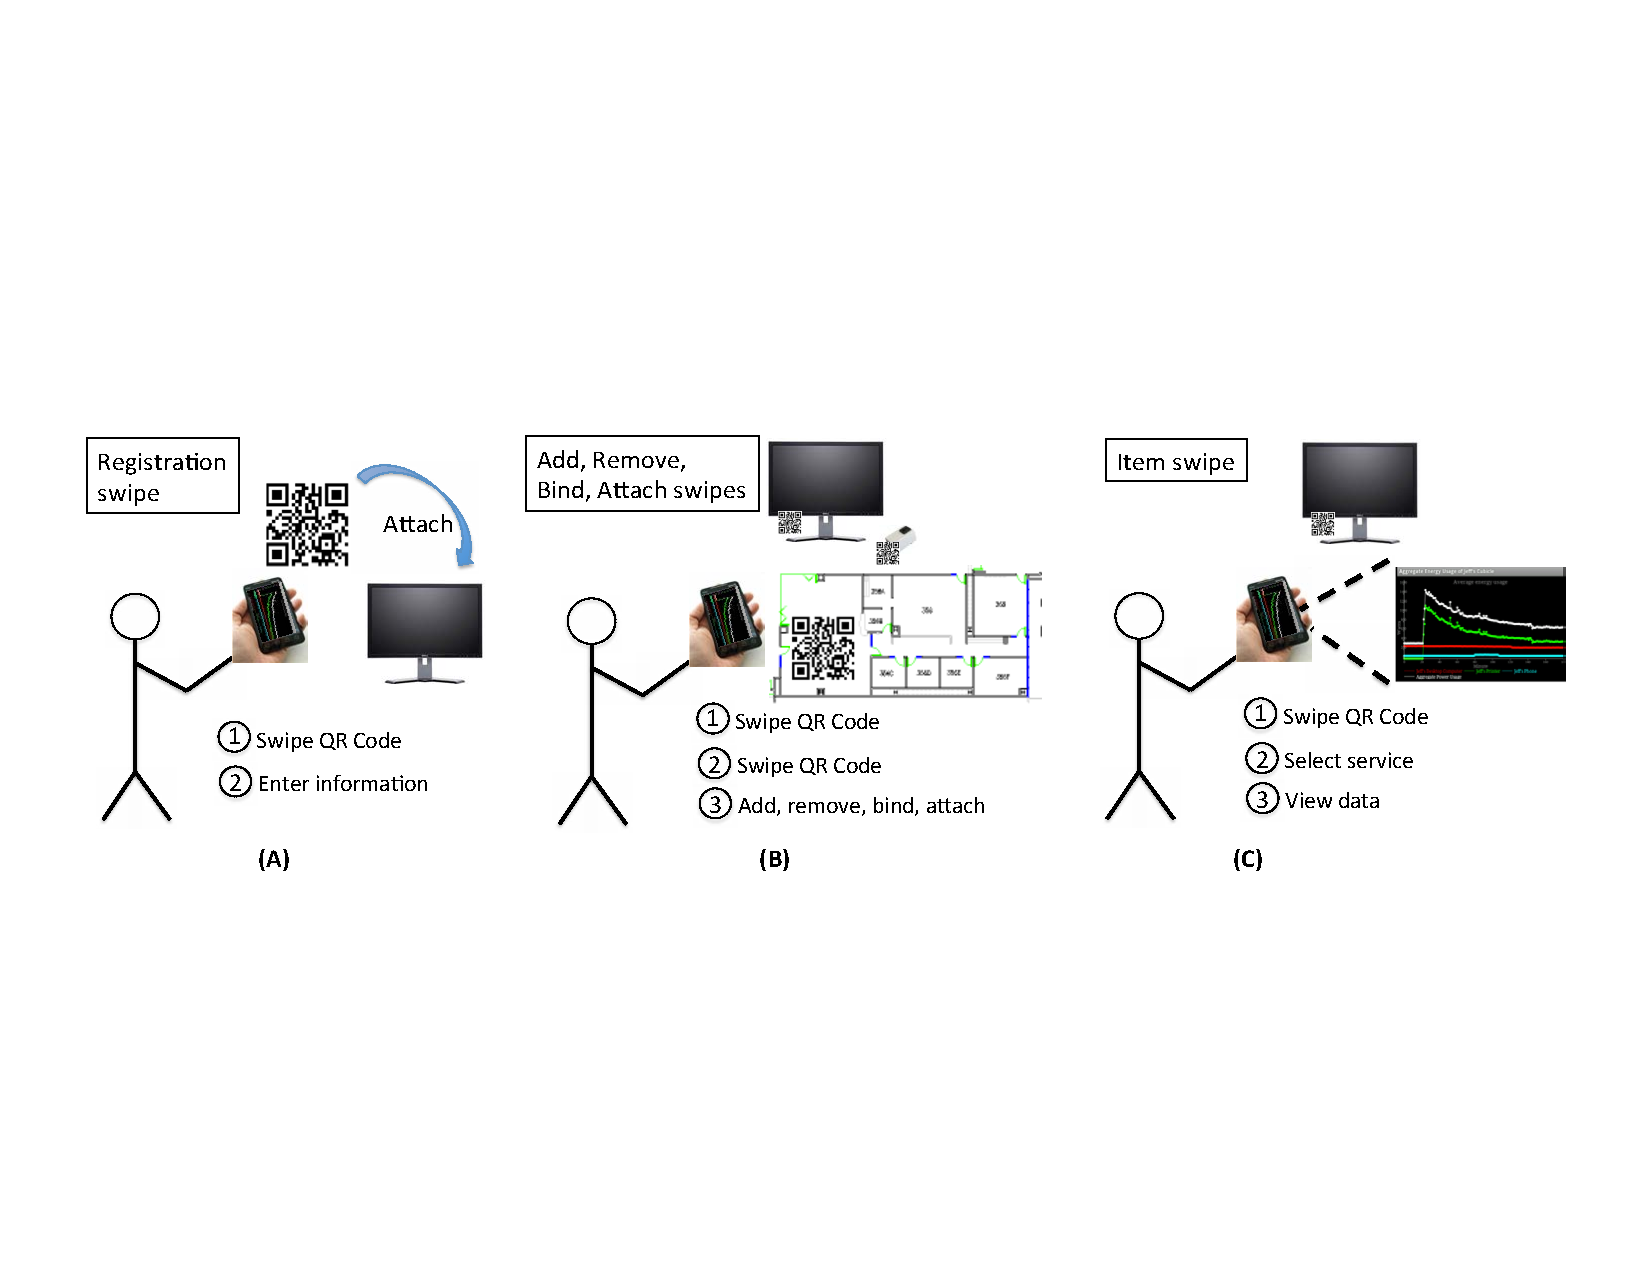
\includegraphics[width=\textwidth]{figs/swipes}
\caption{Gestures. Lorem Ipsum is simply dummy text of the printing and typesetting industry. Lorem Ipsum has 
been the industry's standard dummy text ever since the 1500s, when an unknown printer took a galley of 
type and scrambled it to make a type specimen book.  }
\label{fig:gestures}
\end{center}
\end{figure*}

\begin{figure}[htb!]
\begin{center}
\subfigure[Long QR Code.]{%
            \label{fig:qrcexfirst}
            
\includegraphics[scale=0.148]{figs/qrcexlong}
        }
\subfigure[Minimized QR Code.]{%
            \label{fig:qrcexsecond}
            
\includegraphics[scale=0.35]{figs/qrcex}
        }
\end{center}
\caption{
	The QR code on the left resolves to the same {\tt URL} at the right one, after resolution and
	redirection is complete. 
	The short label resolves to {\tt http://tinyurl.com/6235eyw}.  The second encodes about half
	the characters as the first.
	We used tinyUrl to reduce the QR code image complexity and scan time.
     }%
\label{fig:qrcexcomp}
\end{figure}

\begin{table}
\label{tab:qrscans}
\begin{center}
  \begin{tabular}{| r | c  c | }
    \hline
    			 & {\bf Average (sec) } & {\bf Variance (sec)} \\ \hline
    Short,light & 1.66 & 0.33 \\ \hline
    Short, dark & 2.08 & 0.35 \\ \hline
    Long, light & 2.26 & 0.71 \\ \hline
    Long, dark & 2.82 & 0.50 \\
    \hline
  \end{tabular}
\caption{Shows the time to scan a long QR code versus a short QR code in light and dark conditions (loosely defined).
Notice that short QR codes scan faster and with less variance that long ones.}
\end{center}

\end{table}

Table~\ref{tab:qrscans} shows the results of some simple scanning experiment between the two tags
shown above.  We scanned each QR code under light and dark lighting conditions, off the screen of my laptop.
Each experiment was run 10 times and the table shows the statistical
overview of the results. 
Clearly, scanning the simple QR code under well-lit conditions
performed the best.  The complex QR code under the same condition takes about 28-36\% longer to scan.
On a generic QR code scanner, as used here, there is a portion of the
scan time that is independent of the code complexity.  As these are
more heavily used, this is expected to be reduced substantially and
the difference is acquisition complexity will be even more pronounced.
Perhaps even more important is the variance.  Notice that the variance with the simple QR code is much smaller and
more stable under either condition.  In our experience, {\bf large variance in scan time is a major
problem for complex QR codes}.  Thus we decided to re-design our codes and push more information in the lookup
processes, as network access was more reliable than the focus of the camera on various mobile devices.
Tags are placed on all types of devices in all kinds of locations with varying degrees of lighting.
Simple QR codes are vital for widespread use.

The design choice forced us to examine others that were related.  Not being able to encode much information on 
our QR codes means we are more reliant on the network to provide the bulk of the information, to be very reliable,
and to be widespread enough that disconnection is not problematic.  Moreover, there are a number of clients
that can be used to access and display the information and the tag has to be meaningful for both.
In order to meet these criteria we (1) shrunk {\tt URL}'s using tinyURL~\cite{tinyurl} as a level of 
indirection and 
(2) designed two classes of applications: \emph{shallow} applications, and \emph{deep-inspection} applications.  Shallow
applications interact with the web-application directly while deep-inspection application use
the {\tt URL} of the web application to extract a unique identifier and provide deeper inspection
and update capabilities of the entity-relationship graph.

An example {\tt URL} we used in our deployment is {\tt http://tinyurl.com/6235eyw}.
When this is resolved, we get an empty response in the body, but we use the header to identify the QR code identifier 
that we associate with the item.  The response header looks as follows:
\begin{figure}[htb!]
\begin{center}
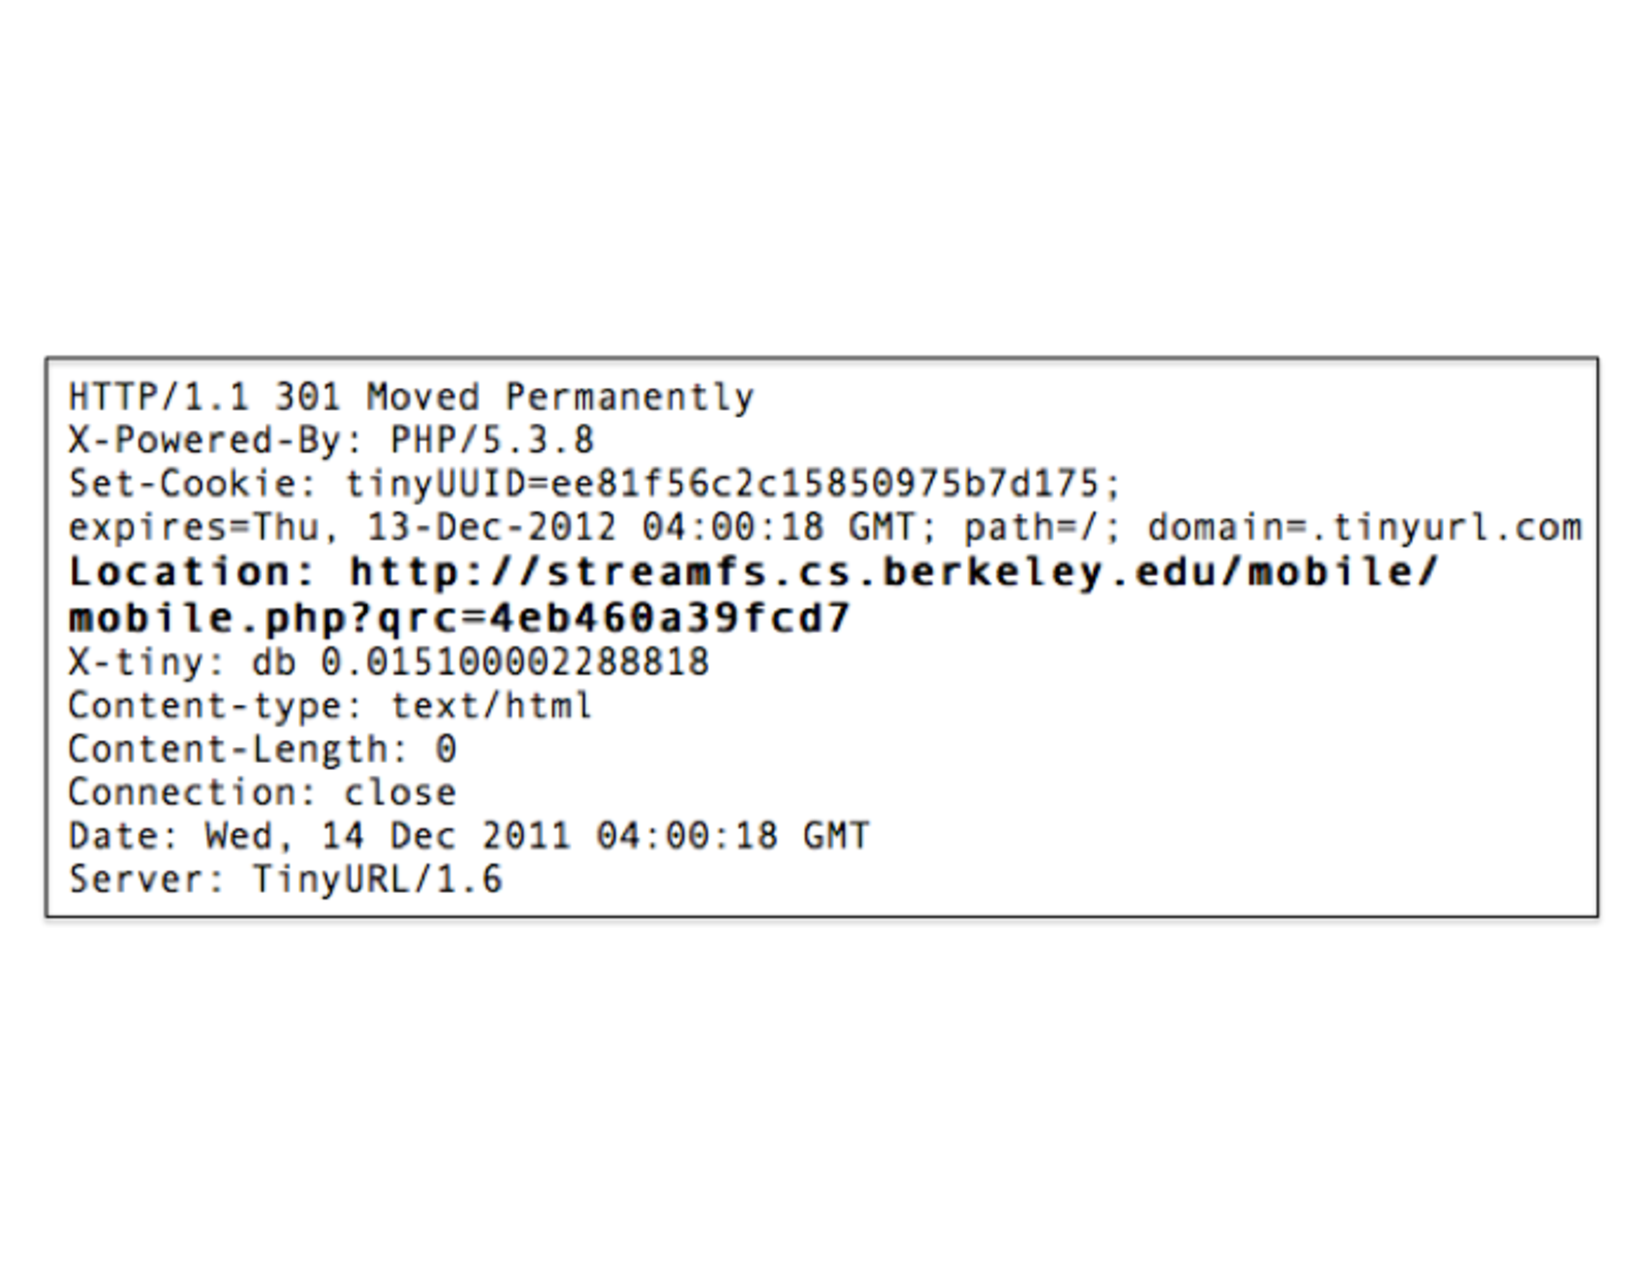
\includegraphics[scale=0.30]{figs/tinyurlhdr}
\caption{The header of the response from the {\tt tinyUrl} when resolving a QR code.  The `Location' attribute
is used to extract the unique identifier for the object this QR code tags.  It is also used to re-direct
users without the phone application to a meaningful web address for the object.}
\label{fig:tinyurlhdr}
\end{center}
\end{figure}

% It provides a web address for users to re-direct to and find information and various read-only services for the object.  However, because
% the {\tt URL} also contains a unqiue identifer \emph{qrc}, it can be used to provide for sophisticated services and capabilities.
% An example is the ability to change the virtual structure of inter-relationship between this object and other objects.  This
% is demonstrated in our energy auditing application discussed in detail in section~\ref{sec:eaudit}.
% Once items are tagged, they can be added and removed by swiping the tag and pressing the button for what you want to do with
% the item.  You also check into locations either explicit with a location-tag swipe or implicitly with an item swipe.

Notice the `Location' attribute in the header.  This is the location of the re-direct.  \emph{Shallow} applications
use the {\tt URL} directly.  The \emph{qrc} {\tt URL} is unqiue identifier for the item that this tag is attached to.
A shallow application can obtain mostly read-only service through our web applications.  For example, we'll see how
to get either item-specific data or item-aggregated data with respect to the user making the request (i.e. the total
energy consumed by \emph{my} devices).  \emph{Deep-inspection} applications are native to the phone, so we can do much
more with the tag.  Our energy auditing application allows you to related the item to other items by maintaining state of swipe
history.  This is more difficult with the web-applicaiton.  We can also use the tag and item information to couple it with
sensor information coming from sensors on the phone itself.  For example, we could determine the direction an object
is pointing by using the phone's directional sensor and negating their direction (i.e. phone is facing east, tag on item must
be facing west).






\subsection{Data management layer}

\subsection{Application layer}


\subsection{Disconnected operation}


\begin{figure}[htb!]
\begin{center}
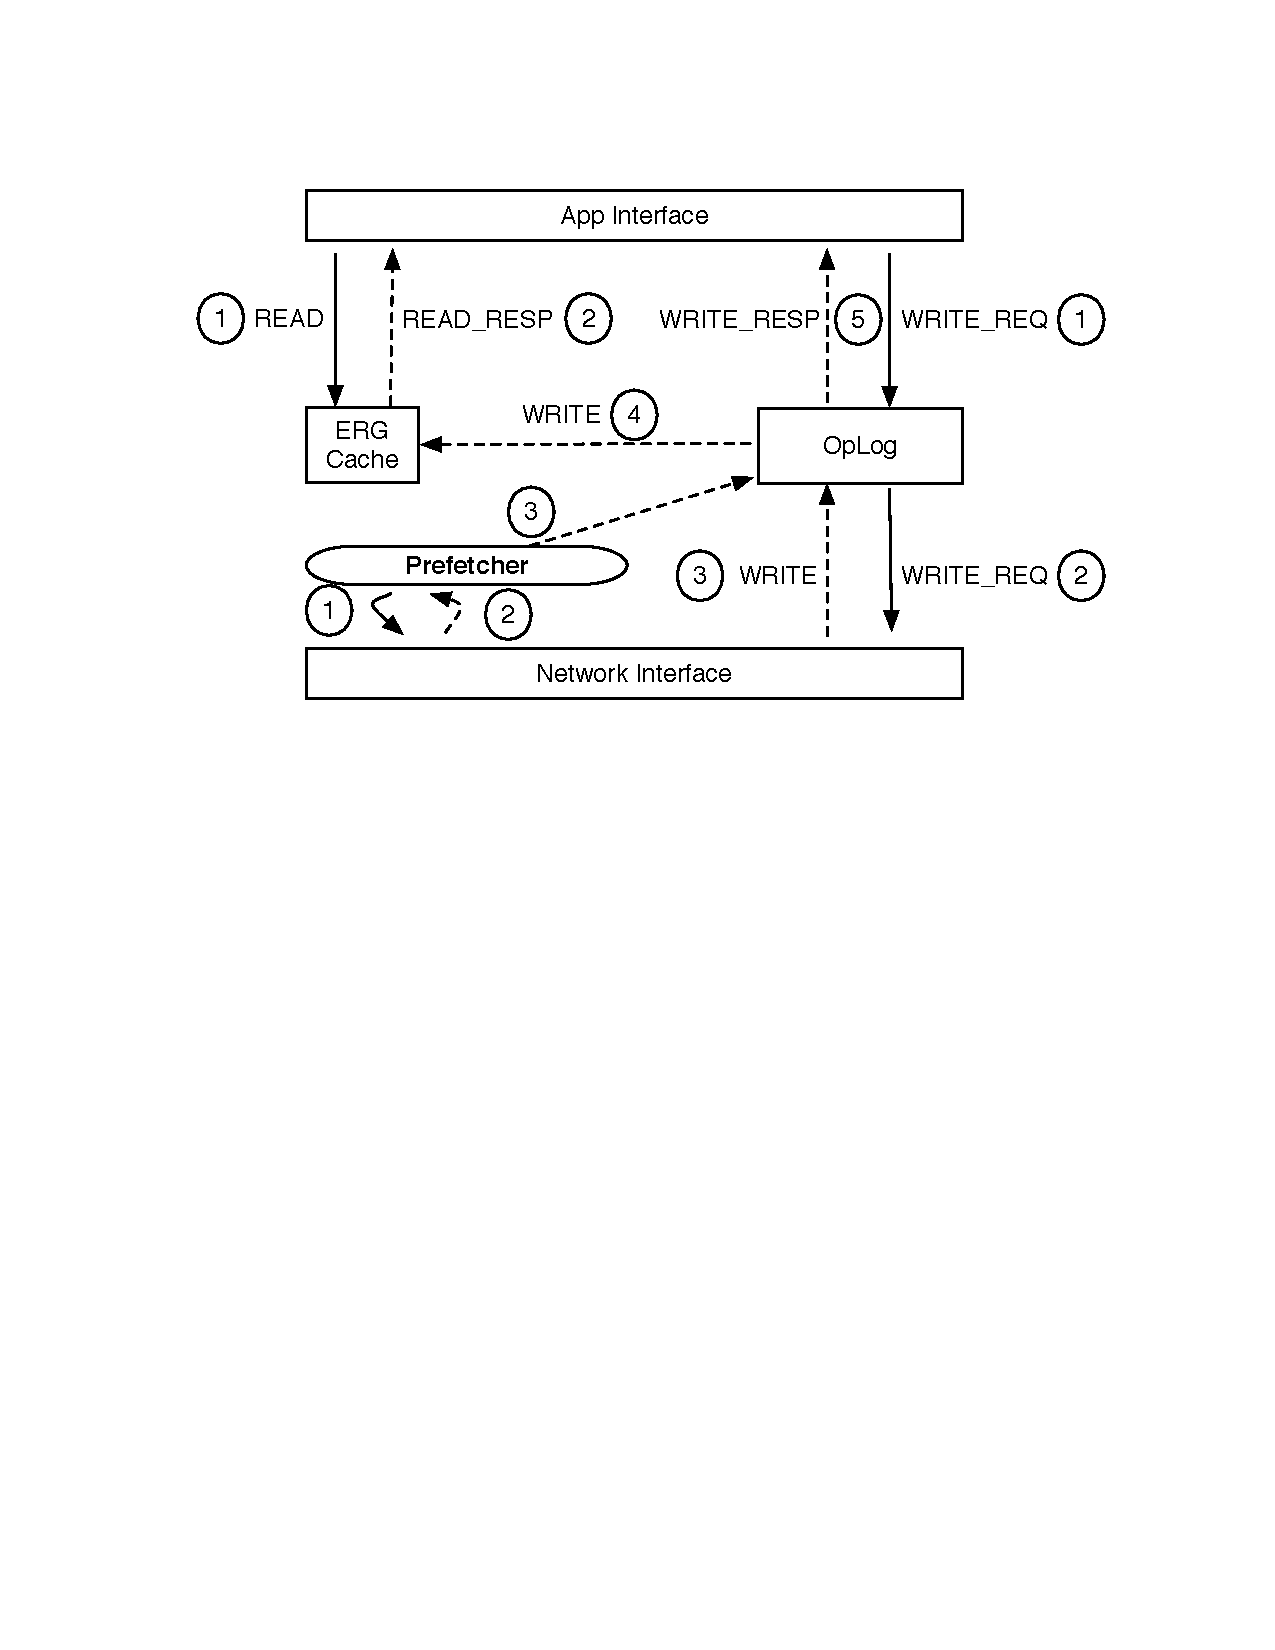
\includegraphics[scale=0.50]{figs/standard_interaction}
\caption{}
\label{fig:interactions}
\end{center}
\end{figure}


\subsection{Swiping gestures}
\label{sec:swipes}

\subsection{Tracking people and things}
There are three major components in our architecture: QR codes, mobile phones, and StreamFS.

How do we evaluate our ability to track people and things?
This is a description evaluation.  We need to describe how the pieces interact.  What will fall out of the description is our strong dependence on occupants/users to give us information about the state of the physical world.  It’ll also fall out that what allows these pieces to fit together is network infrastructure.



\subsection{consistency \& disconnected operations}

The ability to provide real-time analytics for physical data application is driven by 

The consistency and accuracy that we capture about the entities in the world and their relationships and associated metadata.
How those relationships/metadata inform our analytical operations.

Entities in the physical world can be difficult to capture and track over time.  Ideally we’d have a model of the world and the things in it and there would be a mechanism for tracking things that move.  We approximate this mechanism through the combination of QR codes, mobile phones, and people.  Items in the real-world are physically tagged with a QR code that serves as a reference for the “thing” in the physical world.  The mobile phone gives the person a ubiquitous QR code reader.  It also serves to provide the person with services associated with the physical world.

\subsection{Entity-Relationships}
The main aspect we want to capture is entity-relationships between the objects.  Entity relationships are captured through naming and interpreted by the EnergyLens application:

$/path/to/device\_or\_item$

$/path/to/qrc$

$/path/to/space$

$/path/to/taxonomy$

We essentially maintain for separate namespaces and we specify a relationship between them through links between these namespaces.  The relationship is also set by the type of item the path represents.  The types are item, meter, location, system\_device, category, and tag.\\

{\bf Bound-to}\\
When a meter is attached to an item and taking physical measurements associated with that device, we say that the meter is “bound-to” the device.

{\bf Attached-to}\\
When a meter/qr code/item is attached to another meter/qr code/item but NOT taking any physical measurements for that item, we say that the meter/item is “attached-to” the other meter/qr code/item.  QR codes should not be attached to each other and are not accepted by the EnergyLens application.

{\bf Inside-of}\\
When a meter/item is inside a location, we say that the meter/item is “inside-of” that location.

{\bf Type-of}\\
When an item is labeled by as a known, specific, type, we say that the item is a “type-of” thing specified by the its label.


\begin{figure}[htb!]
\begin{center}
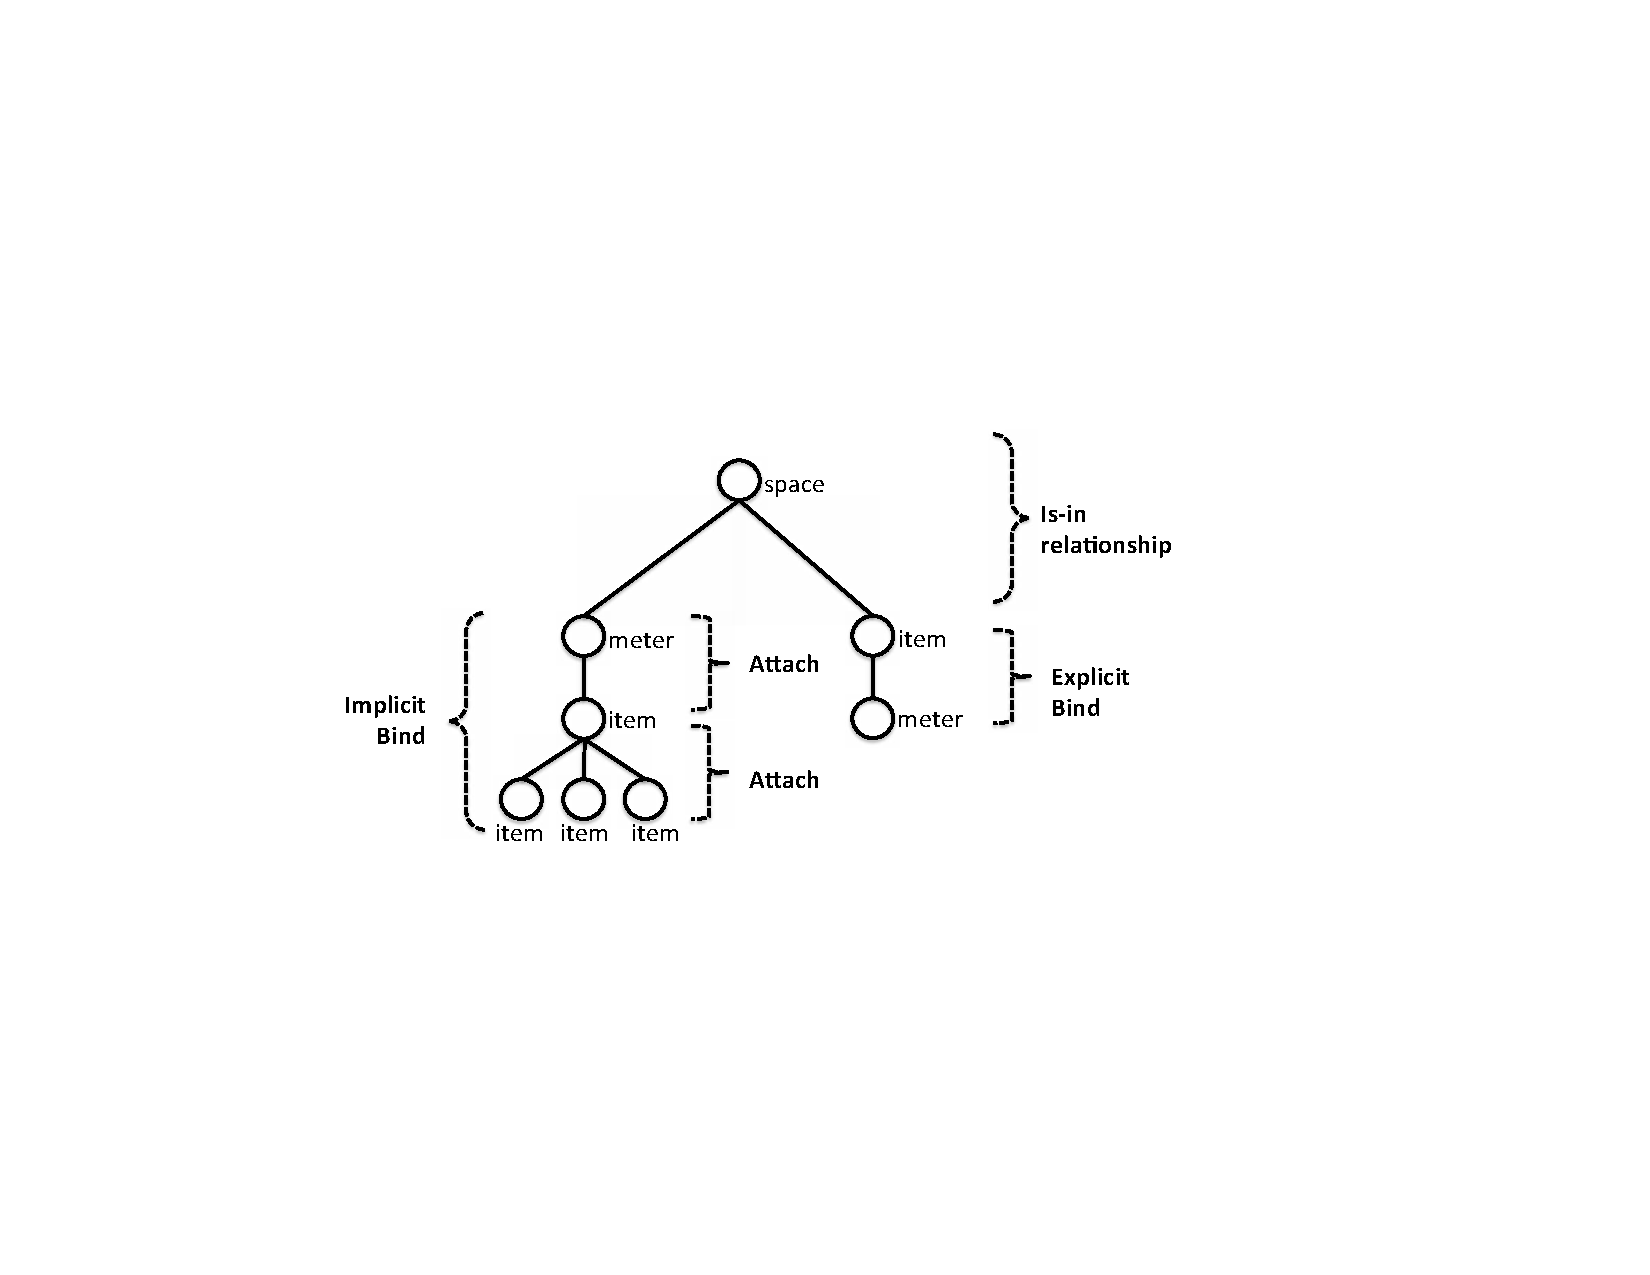
\includegraphics[scale=0.55]{figs/bindattachstructs}
\caption{This diagram shows the relationship capture between the objects and locations in the building for the 
energy audit application.  Children of a space node have an ``is-in'' relationship with the space.  An item
with another item as a child have a ``attached'' relationship and meters attached to items are bound to each other.
Note, this is a \emph{subset} of the relationship diagrams generated across our three applications.}
\label{fig:attachandbind}
\end{center}
\end{figure}

\subsection{Managing consistency while disconnected}

\subsubsection{Caching}
Although network connectivity is theoretically ubiquitous, in practice, this is not always the case.  In order to enable updates while disconnection we need to cache as much of the relevant deployment state as possible.

\subsubsection{Pre-fetching \& The state-change stream}
We should pre-fetch, as the tags inform us about what the user might access next.  What are some things to pre-fetch?  All the paths from the current root to the leaves.  We should also fetch the object associated with each file and for streams, we should fetch 1 hours’ worth of data.  In most cases this means fetching about 200-400 KB of data.

\begin{figure}[htb!]
\begin{center}
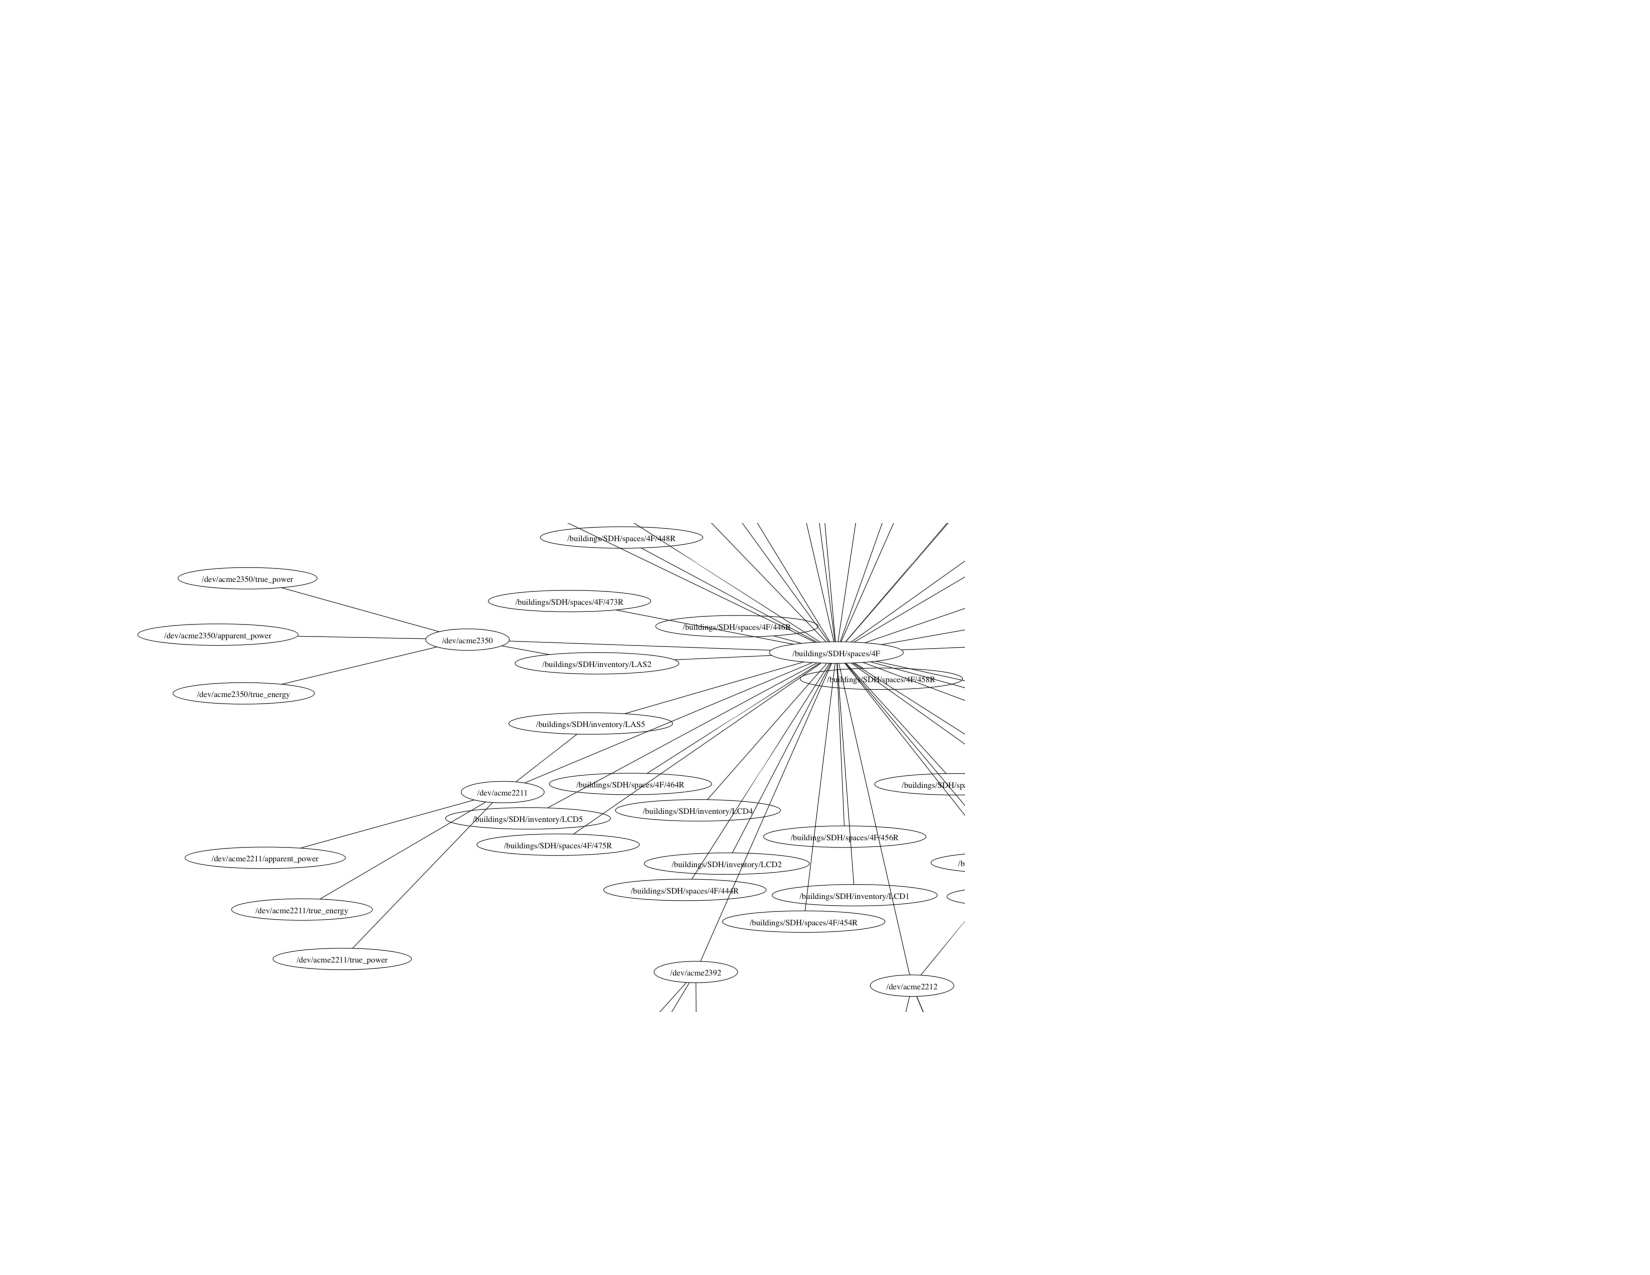
\includegraphics[scale=0.55]{figs/SDH_4F_ERG_closeup}
\caption{A portion of the prefetched entities on the a single floor in our building.  This shows a snapshot of the entity-relationship
graph for that floor.  Each node, link, and associated content is prefetched when the user swipes the floor
tag or anything on that floor.}
\label{fig:sdh_4f_erg}
\end{center}
\end{figure}

\subsection{Conflict resolution}
All transactions are processed in timestamp order, to some rough approximation of the time that the transaction would have been committed.  When a transaction with an earlier timestamp than the last committed transaction is offered, the EnergyLens transaction manager checks if the current transaction conflicts with any previously committed transaction.  This is done by checking if the files that are touched overlap with a transaction that touches the same files and has a transaction timestamp that’s later than the current transaction being offered.  If so the transaction manager rolls back the state of StreamFS, only for the affected files, back to the last transaction before the last commit.  It then commits the offered transaction, adds it to the transaction log, and replays the transaction that was rolled back.  If the operations of the replayed transaction are no longer valid, the transaction fails silently.  Failing silently is acceptable in this context because we want to capture the latest state of the world.  By rejecting the transaction, we are assuming that it was based on false assumptions about the state of the world.  We believe this assumption to be true in most cases.


\subsection{Maintaining, representing, and using physical state and inter-relationships}
In order to provide relevant services, we need to capture the state of the physical environment within the building.  By “relevant”, we mean based on context and inter-relationships.  What are “the relevant services” we’re talking about?

\begin{itemize}
\item Energy analytics on the physical world.
\item How much does this floor consume?
\item What fraction of that is going to the various energy-related categories?  plug-load, hvac, lighting.
\item Personalized energy analytics.
\item Access the the control interface for the physical world.
\end{itemize}

\subsubsection{General approach}
Our approach is to abstractly represents things in the environment as logical entities and to capture their inter-relationships through an entity-relationship graph.  We use the entity relationships to track where objects and things are in the environment, which helps us maintain a more consistent view of the world.  We also use  it to inform our analytical approach and our choice of services to display.

\subsubsection{Consistency management}
Connecting the various components requires ubiquitous connectivity.  Although connectivity is available through the building and the access-point deployment is engineered to minimize dead spots, disconnections still occur (timeout, dead-spots, unsuccessful handoffs).  So, we need to design the system to deal disconnect operation.

Evaluation will be of a protocol description and design rationale described in detail here.
What’s the evaluation exactly?

\begin{enumerate}
\item Time to download the associated contextual information from StreamFS: files, metadata information, data**
\item Conflict resolution examples**
\item Optimizations: Pre-fetching measurements**
\end{enumerate}

\subsection{Real-time analytics}
Discussion.  What to measure here?  Perhaps we discuss the relevant real-time analytics we run?  Will there be space?  For buildsys, include a half page talking about some of the analytics.
% Pub/sub architecture
% time decoupling
% variable time-decoupling achieved through the datastore as a buffer
% synchronization decoupling
% Either the publisher or subscriber run asynchronously.
% space decoupling
% The subscriber doesn’t have an explicit reference to the publisher.
% Programming model for real-time data
% Naming/tagging streams
% Dealing with dynamism through tagging
% Built-in functions for physical data
% heat modeling
% electrical modeling
% mathematical modeling

% Security and privacy
% Discussion.  Various topics related to StreamFS here.  Also some topics related to managing security in StreamFS for doing control.  Include another half page, perhaps.


% * Experiment that we need to run.\\
% ** Code that needs to be written and experiment that needs to be run